\part{}

\section{LED Counter}

In this implementation, the LED decoder circuit will be used to create a 4-bit counter, whose value will be displayed on 
the LEDs through the LED decoder.

This design is hierarchical; both the LED decoder and the counter are autonomous units connected to each other through 
another higher-level unit to create the final circuit.

\subsection{LED Decoder}

The LED Decoder is a combination of LEDs that should display the value of the decoder at any given moment. The decoder 
takes in 4-bits at its input and outputs 7 bits. Essentially, the LED will represent the hexadecimal value of the 4-bits 
as shown in the table below.

\begin{table}[H]
    \centering
    \begin{tabular}{|c|c|}
        \hline
        Binary value & LED value \\ \hline \hline
        0000 & 0 \\ \hline
        0001 & 1 \\ \hline
        0010 & 2 \\ \hline
        0011 & 3 \\ \hline
        0100 & 4 \\ \hline
        0101 & 5 \\ \hline
        0110 & 6 \\ \hline
        0111 & 7 \\ \hline
        1000 & 8 \\ \hline
        1001 & 9 \\ \hline
        1010 & A \\ \hline
        1011 & B \\ \hline
        1100 & C \\ \hline
        1101 & D \\ \hline
        1110 & E \\ \hline
        1111 & F \\ \hline
    \end{tabular}
    \caption{LED Decoder}
    \label{tab:led_decoder}
\end{table}

The construction of the LED Decoder will follow the logic below.

\begin{figure}[H]
    \centering
    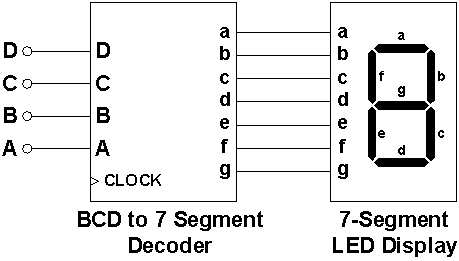
\includegraphics[width=0.5\textwidth]{images/bcd_decoder.png}
    \caption{LED Decoder}
    \label{fig:led_decoder}
\end{figure}

The VHDL code for the LED Decoder is shown here \cref{lst:led_decoder}.

\subsection{Counter}

The counter implemented, is a 4-bit counter that counts from 0 to 15. The increment of the counter is a synchronous
manner, i.e. the counter value is updated only when the clock signal is high. When the counter reaches its maximum value
(15), it resets back to 0 (wrap around). 

The VHDL code for the counter is shown here \cref{lst:counter}. The reset input is used to reset the counter back to 0. 
Besides that, the counter also has a clock input, which is used to increment the counter value. The counter value returned
is a 4-bit value, using a vector.

\subsection{LED Counter}

The LED Counter is a combination of the LED Decoder and the Counter. The LED Counter takes in the clock and reset inputs
from the user and outputs the 7-bit value to be displayed on the LEDs. The LED Counter is a hierarchical design, where
the LED Decoder and the Counter are instantiated as components in the LED Counter.

The VHDL code for the LED Counter is shown here \cref{lst:led_counter}. The LED Counter has a clock and reset input,
which are used to control the counter. The counter value is then passed to the LED Decoder, which returns the 7-bit value
to be displayed on the LEDs. The LED Counter also has a 4-bit output, which is the counter value. 

\subsection{Testbench for LED Counter}

The testbench for the LED Counter is shown here \cref{lst:tb_led_counter}. The testbench instantiates the LED Counter
and provides the clock and reset inputs. The testbench also displays the counter value on the console. The testbench is
run for 100ns, which is enough time for the counter to reach its maximum value and reset back to 0.